\let\negmedspace\undefined
\let\negthickspace\undefined
\documentclass[journal]{IEEEtran}
\usepackage[a5paper, margin=10mm, onecolumn]{geometry}
%\usepackage{lmodern} % Ensure lmodern is loaded for pdflatex
\usepackage{tfrupee} % Include tfrupee package

\setlength{\headheight}{1cm} % Set the height of the header box
\setlength{\headsep}{0mm}     % Set the distance between the header box and the top of the text

\usepackage{gvv-book}
\usepackage{gvv}
\usepackage{cite}
\usepackage{amsmath,amssymb,amsfonts,amsthm}
\usepackage{algorithmic}
\usepackage{graphicx}
\usepackage{textcomp}
\usepackage{xcolor}
\usepackage{txfonts}
\usepackage{listings}
\usepackage{enumitem}
\usepackage{mathtools}
\usepackage{gensymb}
\usepackage{comment}
\usepackage[breaklinks=true]{hyperref}
\usepackage{tkz-euclide} 
\usepackage{listings}
% \usepackage{gvv}                                        
\def\inputGnumericTable{}                                 
\usepackage[latin1]{inputenc}                                
\usepackage{color}                                            
\usepackage{array}                                            
\usepackage{longtable}                                       
\usepackage{calc}                                             
\usepackage{multirow}                                         
\usepackage{hhline}                                           
\usepackage{ifthen}                                           
\usepackage{lscape}
\begin{document}

\bibliographystyle{IEEEtran}
\vspace{3cm}

\title{1-1.5-5}
\author{EE24BTECH11042 - SRUJANA}
% \maketitle
% \newpage
% \bigskip
{\let\newpage\relax\maketitle}

\renewcommand{\thefigure}{\theenumi}
\renewcommand{\thetable}{\theenumi}
\setlength{\intextsep}{10pt} % Space between text and floats


\numberwithin{equation}{enumi}
\numberwithin{figure}{enumi}
\renewcommand{\thetable}{\theenumi}


\textbf{Question}:\\
Find the coordinates of the point which divides the line segment joining the points  $A\vec{(7,-1)}$  and $B\vec{(-3,-4)}$ in the ratio 2 $:$ 3.
\textbf{Solution}:\\
\begin{table}[h!]
	\centering
	\begin{tabular}[12pt]{ |c| |c|}
  \hline
  \textbf{points}&\textbf{coordinates}\\
  \hline
  A & $\brak{7,-1}$\\
  \hline
  B & $\brak{-3,-4}$\\
  \hline
  \end{tabular}

	\label{tab1-1.5-5}
\end{table}
\begin{align}
	A=\myvec{7\\-1} , B=\myvec{-3\\-4}
\end{align}
let C be the point which divides the AB in the ratio $\frac{2}{3} : 1$
\begin{align}
	\implies C=\frac{\frac{2}{3}B+A}{\frac{2}{3}+1}\\
	\implies C=\myvec{3\\\frac{-11}{5}\\}
\end{align}
This can be represented graphically as below
\begin{figure}[h!]
   \centering
   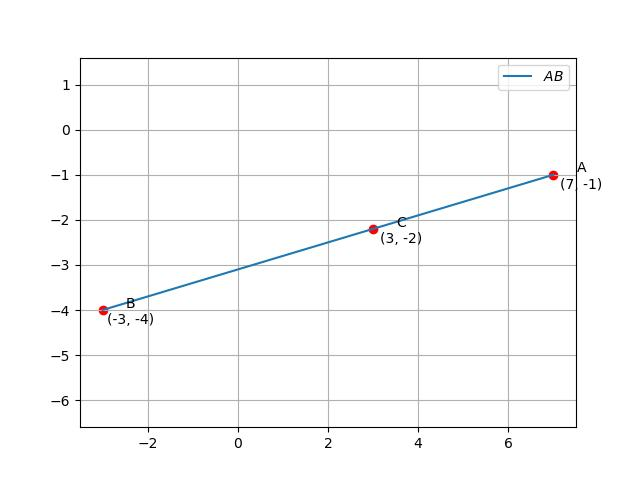
\includegraphics[width=0.7\linewidth]{figs/fig.jpg}
\end{figure}
\end{document}
